\chapter{Monte Carlo Methods}
% Our goal is to estimate value functions and find optimal policies. Monte-Carlo methods require only \textit{experience}--sample sequences of states, actions, and rewards from actual or simulated interaction with an environment. 
Monte Carlo methods are a class of computational algorithms that rely on random sampling to obtain numerical results. In the context of reinforcement learning (RL), Monte Carlo methods are often used to estimate the value of states or state-action pairs in a Markov Decision Process (MDP).


\section{Monte Carlo Prediction (Evaluation)}
% Recall that the value of a state is the expected return starting from that state. An obvious way to estimate it from experience, then, is simply to average the returns observed after visits to that state. As more returns are observed, the average should converge to the expected value. This idea is the core of Monte Carlo methods. 
The goal is to estimate the value of a policy, that is, to learn how much total reward to expect from a policy. 

The most straightforward approach that comes to mind is one I already men- tioned: it’s to run several episodes with this policy collecting hundreds of trajectories, and then calculate averages for every state, just as we did in the bandit environments. This method of estimating value functions is called Monte Carlo prediction (MC).


\subsection{First Visit vs. Every Visit}
Suppose we wish to estimate $v_\pi(s)$, the value of a state $s$ under policy $\pi$, given a set of episodes obtained by following $\pi$ and passing through $s$. Each occurrence of state $s$ in an episode is called a visit to $s$. 

\paragraph{The first-visit MC} method estimates $v_\pi(s)$ as the average of the returns following first visits to $s$, whereas \textit{the every-visit MC} method averages the returns following all visits to $s$.

\begin{itemize}
	\item First visit MC treats each trajectory as an i.i.d., sample of $v(s)$.
	\item For instance, we have two example episodes, 
		\begin{itemize}
			\item $A, 3\to A, 2\to B, -4\to A, 4\to B, -3$.
			\item $B, -2\to A, 3\to B, -3$.
		\end{itemize} 
	\item Each number next to the states are reward. Let's say discount factor is 1 and we want to compute $V(A)$, then the first visit MC computes a return by summing all the rewards ($G\leftarrow \gamma G + R_{t+1}$) coming after the first visit to the state $A$. Therefore, we can't have more than one summation term for each episode for a state. In sum,
	\begin{itemize}
		\item For the first episode: $3+2-4+4-3=2$.
		\item For the second episode: $3-3=0$.
		\item Thus, $V(A) = (2+0)/2=1$.
		\item It must be noted that if an episode doesn't have an occurrence of `$A$', it won't be considered in the average. Hence if a 3rd episode is given like $B,3\to B,3\to terminate$ existed, still $V(A)=1$.
	\end{itemize}
\end{itemize}

\begin{figure}[h]
	\centering
	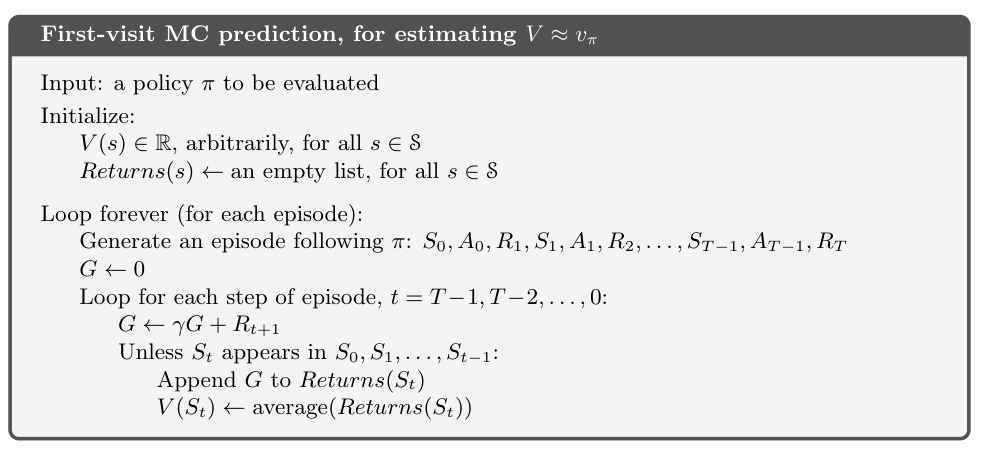
\includegraphics[scale=0.5]{./images/first_visit_mc.png}
	\caption{First-visit MC prediction algorithm.}
	\label{fig:first_visit_mc}
\end{figure}

\paragraph{Every visit MC} method averages the returns following \textbf{all visits} to $s$.
\begin{itemize}
	\item Here, we would be creating a new summation term adding all rewards coming after every occurrence of `$A$'(including that of $A$ as well).
		\begin{itemize}
			\item From 1st episode: $(3+2-4+4-3)+(2-4+4-3)+(4-3)=2-1+1$
			\item From 2nd episode: $(3-3)=0$
			\item As we got 4 summation terms, we will be averaging using $N=4$ \ie
			\item $V(A)=(2-1+1+0)/4=0.5$
		\end{itemize}
\end{itemize}



\section{Monte Carlo Control}
$$\pi_0\xrightarrow{\,E\,} q_{\pi_0} \xrightarrow{\,I\,} \pi_0\xrightarrow{\,E\,} q_{\pi_0}\xrightarrow{\,I\,}\cdots \xrightarrow{\,I\,} \pi_*\xrightarrow{\,E\,} q_{\pi_*},$$
\begin{itemize}
	\item $\pi_0$: arbitrary policy.
	\item Policy improvement is done by making the policy greedy with respect to the current value function (action-value function). 
	\item For any action-value function $q$, the corresponding greedy policy is the one that, for each $s\in \mathcal{S}$, deterministically chooses an action with maximal action-value:
		$$\pi(S) = \argmax_a q(s,a).$$
	\item Policy improvement then can be done by constructing each $\pi_{k+1}$ as the greedy policy with respect to $q_{\pi_k}.$
	\item By \Cref{thrm:policy_improvement}, each $\pi_{k+1}$ is uniformly better than $\pi_k$ or just as good as $\pi_k$.
\end{itemize}


\section{On-Policy vs. Off-Policy}
%Monte Carlo prediction (or evaluation) is used to evaluate the value of a given policy, while Monte Carlo control is for finding the optimal policy when such a policy is not given. There are two categories of MC control:
\paragraph{On-policy} learns about the optimal policy by executing the policy and evaluating and improving it.  
\begin{itemize}
	\item Learning to be great by itself.
	\item The agent learns from the experiences it gathers while following its current policy.
	\item The policy is typically denoted by $\pi$.
	\item The learning process is directly tied to the policy being used for action selection.
	\item Examples of on-policy algorithms include REINFORCE (Monte Carlo Policy Gradient) and Proximal Policy Optimization (PPO).
	\end{itemize}

\paragraph{Off-policy} learns about the optimal policy by using data generated by another policy. 
\begin{itemize}
	\item Learning from others.
	\item The agent can learn from historical data, which may have been generated by an older policy.
	\item The policy used for learning is not necessarily the one used for action selection.
	\item The data collected can be more efficiently reused for learning new policies.
	\item Examples of off-policy algorithms include Q-learning, Deep Q Networks (DQN), and Actor-Critic methods.
\end{itemize}


\paragraph{Exploration-Exploitation Trade-off}
\begin{itemize}
	\item On-policy algorithms often struggle with exploration because they are committed to following their current policy, which may not explore the state space efficiently.
	\item Off-policy algorithms can be more sample-efficient in exploration as they can learn from a mixture of data from different policies.
\end{itemize}

\paragraph{Data Efficiency}
\begin{itemize}
	\item Off-policy algorithms can potentially be more data-efficient since they can reuse past experiences collected by any policy.
	\item On-policy algorithms typically require more samples to update the policy effectively.
\end{itemize}
    
\paragraph{Stability and Convergence}
\begin{itemize}
	\item On-policy algorithms can be more stable because they are directly optimizing the policy they are following.
	\item Off-policy algorithms might face challenges related to the stability of learning, especially when dealing with function approximation, as is often the case with deep learning.
\end{itemize}
    
Both on-policy and off-policy algorithms have their strengths and weaknesses, and the choice between them depends on the specific requirements and characteristics of the problem at hand.

\section{Exploration-Exploitation Trade-off}
The more episodes are collected, the better, but there is a problem. If the algorithm for policy improvement always updates the policy greedily, meaning it takes only actions leading to immediate reward, actions and states not on the greedy path will not be sampled sufficiently, and potentially better rewards would stay hidden from the learning process.

Essentially, we are forced to make a choice between making the best decision given the current information or start exploring and finding more information. This is also known as the Exploration vs. Exploitation Dilemma.

We are looking for something like a middle ground between those. Full-on exploration would mean that we would need a lot of time to collect the needed information, and full-on exploitation would make the agent stuck into a local reward maximum. There are two approaches to ensure all actions are sampled sufficiently called on-policy and off-policy methods.



\subsection{On Policy}
On-policy methods solve the exploration vs exploitation dilemma by including randomness in the form of a policy that is soft, meaning that non-greedy actions are selected with some probability. These policies are called $\epsilon$-greedy policies as they select random actions with an $\epsilon$ probability and follow the optimal action with $1-\epsilon$ probability

Since the probability of selecting from the action space randomly is $\epsilon$, the probability of selecting any particular non-optimal (non-greedy) action is $\epsilon/|\mathcal{A}(s)|$. The probability of following the optimal action will always be slightly higher, however, because we have a $1 - \epsilon$ probability of selecting it outright and $\epsilon/ |\mathcal{A}(s)|$ probability of selecting it from sampling the action space \footnote{Since the greedy (or optimal) action can be selected by either 1-$\epsilon$ or $\epsilon/ |\mathcal{A}(s)|$, $a_1=\epsilon/\mathcal{A}(s),a_2=\epsilon/\mathcal{A}(s),\cdots,a_{best}=1-\epsilon+\epsilon/\mathcal{A}(s),a_n = \epsilon/\mathcal{A}(s)$}
$$P(a_t^{*}) = 1 - \epsilon+\epsilon/ |\mathcal{A}(s)|.$$
It is also worth noting that because the optimal action will be sampled more often than the others making on-policy algorithms will generally converge faster but they also have the risk of trapping the agent into a local optimum of the function.

%On-Policy learning algorithms are the algorithms that evaluate and improve the same policy which is being used to select actions. That means we will try to evaluate and improve the same policy that the agent is already using for action selection. In short , [Target Policy == Behavior Policy]. Some examples of On-Policy algorithms are Policy Iteration, Value Iteration, Monte Carlo for On-Policy, Sarsa, etc.

\subsection{Off Policy}

All learning control methods face a dilemma: They seek to learn action values conditional on subsequent \textit{optimal} behavior, but they need to behave non-optimally in order to explore all actions (to find the optimal actions). How can they learn about the optimal policy while behaving according to an exploratory policy? The on-policy approach in the preceding section is actually a compromise. It learns action values not for the optimal policy, but for a near-optimal policy that still explores. A more straightforward approach is to \textbf{leverage two policies}, one that is learned about and that becomes the optimal policy, and one that is more exploratory and is used to generate behavior. The policy being learned about is called the \textit{target policy}, and the policy used to generate behavior is called the \textit{behavior policy}. In this case we say that learning is from data ``off'' the target policy, and the overall process is termed \textit{off-policy learning}.

Suppose we wish to estimate $v_\pi$ or $q_\pi$, but all we have are episodes following another policy $b$, where $b\neq \pi$. In this case, $\pi$ is the target policy, $b$ is the behavior policy, and both policies are considered fixed and given. 

In order to use episodes from $b$ to estimate values for $\pi$, we require that every action taken under $\pi$ is also taken, at least occasionally, under $b$. That is, we require that $\pi(a|s) > 0$ implies $b(a|s) > 0$. This is called the assumption of \textit{coverage}. It follows from coverage that $b$ must be stochastic in states where it is not identical to $\pi$. The target policy $\pi$, on the other hand, may be deterministic, and, in fact, this is a case of particular interest in control applications. In control, the target policy is typically the deterministic greedy policy with respect to the current estimate of the action-value function. This policy becomes a deterministic optimal policy while the behavior policy remains stochastic and more exploratory, for example, an $\epsilon$-greedy policy. %In this section, however, we consider the prediction problem, in which ⇡ is unchanging and given.

Almost all off-policy methods utilize \textit{importance sampling}, a general technique for \textbf{estimating expected values under one distribution given samples from another}. We apply importance sampling to off-policy learning by weighting returns according to the relative probability of their trajectories occurring under the target and behavior policies, called the \textit{importance-sampling ratio}. Given a starting state $S_t$, the probability of the subsequent state-action trajectory, $A_t, S_{t+1}, A_{t+1},\cdots,S_T$, occurring under any policy $\pi$ is 
\begin{align*}
	P(A_t, S_{t+1}, A_{t+1},\cdots,S_T)&= \pi(A_t|S_t)p(S_{t+1}|S_t,A_t)\pi(A_{t+1}|S_{t+1})\cdots(S_T|S_{T-1},A_{T-1})\\ 
	&= \prod_{k=t}^{T-1}\pi(A_k|S_k)p(S_{k+1}|S_k,A_k),
\end{align*}
where $p$ here is the state-transition probability function. Thus, the relative probability $\rho$ of the trajectory under the target ($\pi$) and behavior policies ($b$) is 
\begin{align*}
	\rho_{t:T-1} &=  \frac{\prod_{k=t}^{T-1}\pi(A_k|S_k)p(S_{k+1}|S_k,A_k)}{ \prod_{k=t}^{T-1}b(A_k|S_k)p(S_{k+1}|S_k,A_k)}\\
	&= \prod_{k=t}^{T-1}\frac{\pi(A_k|S_k)}{b(A_k|S_k)}.
\end{align*}
The importance sampling ratio ends up depending only on the two polices and the sequence, not on the MDP's state-transition probability.

Recall that we wish to estimate the expected returns under the target policy, but all we have are returns $G_t$ from the behavior policy, which results in 
\begin{align*}
	\mathbb{E}[G_t|S_t=s] = v_b(s).
\end{align*}

So, the ratio $\rho_{t:T-1}$ transforms the returns
\begin{align*}
	\mathbb{E}[\rho_{t:T-1} G_t|S_t=s] = v_\pi(s).
\end{align*}

\section{Temporal-Difference Learninig}
One of the central ideas of reinforcement learning is temporal-difference (TD) learning. TD learning is a combination of Monte Carlo ideas and dynamic programming (DP) ideas. Like Monte Carlo methods, TD methods can learn directly from raw experience without a model of the environment's dynamics. Like DP, TD methods update estimates based in part on other learned estimates, without waiting for a final outcome (they bootstrap). 

One of the main drawbacks of MC methods is the fact that the agent has to wait until the end of an episode when it can obtain the actual $G_t$. Then, it uses that return as a target for $V(S_t)$.


The core of TD learning is the Temporal Difference (TD) error, denoted as $\delta_t$, which represents the difference between the estimated value of a state at time $t$ and the estimated value at time $t+1$. It is calculated as the difference between the reward at time $t+1$ and the discounted estimate of the value function at time $t$.

Constant-$\alpha$ MC:
$$V(S_t) \leftarrow V(S_t)+ \alpha \Big[G_t-V(S_t)\Big] $$

One-step TD (or TD(0)):
$$V(S_t) \leftarrow V(S_t)+ \alpha \Big[\underbrace{R_{t+1}+\gamma V(S_{t+1})-V(S_t)}_{\text{TD error, $\delta$}}\Big] $$

To clarify the difference, let's consider a simple example of a grid-world navigation task. 

\paragraph{MC Method} The agent explores the grid-world and reaches a target goal ($S_9$). The episode ends, and the agent receives a reward of +1. At the end of the episode, the agent updates the value of each visited state based on the observed return. If the trajectory is $S_1\to S_2 \to \cdots\to S_9$, then the value update for each visited state would be based on the return of +1.

\paragraph{TD Learning} The agent starts at $S_1$, moves to $S_2$, and receives a reward of $-0.1$ for the movement. The agent updates the value of $S_1$ based on the observed TD error, which is the immediate reward plus the discounted estimate of the next state. If the agent moves right from $S_1$ to $S_2$, the update for $S_1$ would be based on $R_{move}+\gamma V(S_2)$.

\begin{itemize}
	\item Monte Carlo:
		\begin{itemize}
			\item Pros: Unbiased estimate of value functions.
			\item Cons: Requires complete episodes, might be computationally expensive.
		\end{itemize}
	\item Temporal Difference:
		\begin{itemize}
			\item Pros: Updates at each time step, more sample-efficient.
			\item Cons: Potential bias due to bootstrapping.
		\end{itemize}
\end{itemize}
In summary, in the grid-world example, Monte Carlo methods would update values based on complete episodes, whereas TD learning would update values at each time step. The choice depends on the nature of the task, the availability of information, and the computational resources.

\begin{lstlisting}[language=Python]
import numpy as np
import random

def random_walk_environment(state):
    """
    Given the current state (1..5), this environment transitions left or right 
    with equal probability and returns the next state, as well as the reward.
    
    Args:
        state (int): Current non-terminal state, 1 <= state <= 5.
    
    Returns:
        next_state (int): Next state in {0,1,2,3,4,5,6}.
        reward (float): Reward for the transition.
    """
    # Action: move left (prob=0.5) or right (prob=0.5)
    action = random.choice([-1, +1])
    next_state = state + action

    # If next_state == 6, reward = +1; if next_state == 0, reward = 0
    # For states 1..5, reward = 0
    if next_state == 6:
        reward = 1.0
    else:
        reward = 0.0
    
    return next_state, reward


def td_zero_random_walk(num_episodes=1000, alpha=0.1, gamma=1.0):
    """
    Perform TD(0) to evaluate the value function V(s) for the random walk example.
    
    Args:
        num_episodes (int): Number of episodes to run.
        alpha (float): Step-size / learning rate.
        gamma (float): Discount factor (set to 1.0 in the classic random walk).
    
    Returns:
        V (np.array): Learned value function estimates V(s) for states s in [0..6].
                      Terminal states 0 and 6 stay at V=0 by definition.
    """
    # We track V(s) for states 0..6, but 0 and 6 are terminal.
    # Initialize with zeros (you could initialize them differently).
    V = np.zeros(7)

    for episode in range(num_episodes):
        # Start each episode in the middle state (often chosen as 3 in the random walk)
        state = 3

        # Continue until we reach a terminal state
        while state not in [0, 6]:
            next_state, reward = random_walk_environment(state)

            # TD(0) update:
            # V[s] <- V[s] + alpha * [R + gamma * V[s'] - V[s]]
            V[state] = V[state] + alpha * (reward + gamma * V[next_state] - V[state])

            state = next_state

    return V

if __name__ == "__main__":
    # Set random seed for reproducibility (optional)
    random.seed(42)
    np.random.seed(42)

    # Run TD(0) for 1000 episodes
    num_episodes = 1000
    alpha = 0.1
    V_estimates = td_zero_random_walk(num_episodes, alpha)

    print(f"Value Function Estimates after {num_episodes} episodes:")
    for s in range(7):
        print(f"V({s}) = {V_estimates[s]:.3f}")
\end{lstlisting}


\subsection{Q-learning: Off-policy TD Control}

$$Q(S_t, A_t) \leftarrow Q(S_t, A_t)+ \alpha \Big[R_{t+1}+\gamma \max_a Q(S_{t+1}, a)-Q(S_t, A_t)\Big] $$

\begin{itemize}
	\item Off-policy. For instance, we can sample an action $A_t$ from a $\epsilon$-greedy policy. 
	\item Update Q for each step.
	\item Maximization bias in $Q$-learning
\end{itemize}

\subsection{Sarsa: On-policy TD Control}
$$Q(S_t, A_t) \leftarrow Q(S_t, A_t)+ \alpha \Big[R_{t+1}+\gamma Q(S_{t+1}, A_{t+1})-Q(S_t, A_t)\Big] $$
\begin{itemize}
	\item On-policy agorithm, unlike $Q$-learning, we sample both $A_t$ and $A_{t+1}$ from another policy like $\epsilon$-greedy policy. 
\end{itemize}


\subsection{Double Q-learning}

Randomly select $Q_1$ or $Q_2$.

$$Q_1(S_t, A_t) \leftarrow Q_1(S_t, A_t)+ \alpha \Big[R_{t+1}+\gamma \max_a Q_2(S_{t+1}, a^*)-Q_1(S_t, A_t)\Big], $$
where $a^*$ is 
$$a^* = \argmax_a Q_1(s',a).$$

$$Q_2(S_t, A_t) \leftarrow Q_2(S_t, A_t)+ \alpha \Big[R_{t+1}+\gamma \max_a Q_1(S_{t+1}, a^*)-Q_2(S_t, A_t)\Big], $$
where $a^*$ is 
$$a^* = \argmax_a Q_2(s',a).$$
